\section{Evaluation}

A large challenge in creating quality measures is the
problem of evaluating the performance of the measure.
``Quality'' is an imprecise notion by itself, because it
necessarily must be evaluated with respect to some attribute.
For example, within the Wikipedia we might evaluate the quality
of a contribution along any of these dimensions:
\begin{itemize}
\item grammar
\item diction
\item neutral point of view
\item factual correctness
\end{itemize}
Our text and edit longevity measures try to go one step
further into the fuzzy world of human evaluations by using
later edits as a basis for inferring sentiment about earlier edits.
Is this a valid inference to make?
How can such a question be answered?

The surest way to measure sentiment would be to interview
users as they are making edits to the Wikipedia and documenting
their thought processes as they read an article and make the
decision to edit an article --- but this would require an enormous
effort to collect enough data for performance evaluation.
We propose that we can grossly measure the sentiment of the
community by recognizing that there is a generally agreed upon
standard of articles being of ``encyclopedic quality''
which allows people to recognize vandalism when they see it.
Accepting that premise allows us to use the PAN-WVC-10
corpus~\cite{Potthast2010a} as a manually annotated data set for
such an evaluation.

The PAN-WVC-10 corpus was used to compare the performance of
solutions for the 1st International Competition on Wikipedia
Vandalism Detection (PAN-WVD~2010)~\cite{Potthast2010b}.
We use it in a similar way here to compare how well our quality
measures are able to predict vandalism within the corpus,
but with an important distinction:
we use information ``from the future'' to calculate our
quality values for the annotated revisions.
Standard vandalism detection tools make their determination
immediately as the edit is made, so that any vandalism can be
quickly repaired by others.
The necessity for a quick classification precludes waiting
for future edits or rating to corroborate the edit being judged;
we term this variation of the problem \textit{immediate vandalism detection}.
By definition, our two longevity metrics use later edits to
measure the quality of the revision being judged; we call
this the \textit{historical vandalism detection} problem.
Historical vandalism detection has its own set of important
applications, such as selecting high quality revisions for
DVD compilations or for presentation to school children.

The PAN-WVC-10 corpus contains 32,439 edits, where each revision was
manually reviewed by at least three annotators to assign a label
of either ``regular'' or ``vandalism.''
We used the dump of the English Wikipedia from January 30, 2010
to extract the text of each annotated revision, along with the revision
before and the ten filtered revisions following so that we could compute
our text longevity and edit longevity measures for each annotated edit.

We used the straight-forward transformation to convert
each quality score from its normal range into the range
$[0,1]$, to be interpreted as a probability that the named
revision was the result of vandalism.
As in the PAN-WVD~2010 competition~\cite{Potthast2010b}, we use the
\texttt{perf}\footnote{\url{http://osmot.cs.cornell.edu/kddcup/software.html}}
package to evaluate the performance of our quality measures
by computing the areas under the receiver operating characteristic
curve \footnote{\url{http://en.wikipedia.org/wiki/Receiver_operating_characteristic}},
and the precision-recall curve.

\subsection{Difference Algorithms}

Each formula for edit distance we have defined so far is calculated
from the operations within the edit script describing the transformation
from the source revision to the target revision.
This edit script is highly dependent on the algorithm used to
compute the difference between the revisions.
To provide a more complete picture of how the choice of difference
algorithm affects the performance of the quality measures,
we present an evaluation of some variations of the algorithms;
the OCaml source representing these algorithms appears
in Appendix \ref{app:diffsrc-ocaml}.
The list of algorithm variations that we tried are as follows:
%
\begin{description}

\item[\textbf{diff1}]
    Implementation of the Tichy greedy algorithm, including optimizations
    suggested by Obst and Reichenberger.
    \begin{description}
    \item[Includes:]
        \textbf{min wordlen}, \textbf{max matches},
    \item[Excludes:]
        \textbf{header/trailer}.
        \textbf{longest match}, \textbf{prev matches}.
    \end{description}

\item[\textbf{diff2}]
    Implementation of the Tichy greedy algorithm, including optimizations
    suggested by Obst and Reichenberger.  Also includes the
    \textbf{header/trailer} optimization.
    \begin{description}
    \item[Includes:]
        \textbf{min wordlen}, \textbf{max matches}, \textbf{header/trailer}
    \item[Excludes:]
        \textbf{longest match}, \textbf{prev matches}.
    \end{description}

\item[\textbf{diff3}]
    The \textbf{prev matches} optimization is only applicable
    on top of the \textbf{longest match} optimization.
    On average, it has significantly reduced memory requirements
    over \textbf{longest match} implemented with an associative array
    to track matches made so far.
    %
    \begin{description}
    \item[Includes:]
	\textbf{min wordlen}, \textbf{max matches},
	\textbf{header/trailer}, \textbf{longest match}.
    \item[Excludes:]
	\textbf{prev matches}.
    \end{description}

\item[\textbf{diff4}]
    This variation of our difference algorithm explores another
    combination of optimizations.
    We believe that the \textbf{header/trailer} optimization generates
    an edit script which is closer to a human understanding of text
    differencing, so that we expect this variation to perform worse
    than \textbf{diff5}.
    %
    \begin{description}
    \item[Includes:]
	\textbf{min wordlen}, \textbf{max matches}, \textbf{longest match},
	\textbf{prev matches}.
    \item[Excludes:]
	\textbf{header/trailer}.
    \end{description}

\item[\textbf{diff5}]
    %
    \begin{description}
    \item[Includes:]
	\textbf{min wordlen}, \textbf{max matches},
	\textbf{header/trailer}, \textbf{longest match},
	\textbf{prev matches}.
    \item[Excludes:] \textit{none}.
    \end{description}

\item[\textbf{diff6}] This is the original difference algorithm
    for comparing two revisions in the WikiTrust system, as
    described in~\cite{Adler2007}.
    %
    \begin{description}
    \item[Includes:]
	\textbf{min wordlen}, \textbf{max matches}, \textbf{longest match},
	\textbf{prev matches}.
    \item[Excludes:]
	\textbf{header/trailer}.
    \end{description}
    This version of the difference algorithm includes other
    functionality not described here.
    The source code implementing this version is available from
    Github,\footnote{\url{http://www.github.com/collaborativetrust/WikiTrust}}
    and corresponds to the function \texttt{edit\_diff\_core} in
    file \texttt{chdiff.ml}.

\item[\textbf{diff7}]
    This is the difference algorithm currently running on the live
    production
    WikiTrust system.
    It is the same as \textbf{diff6}, with the addition of the
    \textbf{header/trailer} optimization.
    %
    \begin{description}
    \item[Includes:]
	\textbf{min wordlen}, \textbf{max matches}, \textbf{longest match},
	\textbf{prev matches}, \textbf{header trailer}.
    \item[Excludes:] \textit{none}.
    \end{description}
    %
    It is able to process user reputations and text trust fast enough
    to keep up with each change being made to the English Wikipedia.
    The source code implementing this version
    corresponds to the function \texttt{edit\_diff} in
    file \texttt{chdiff.ml}, available via Github.

\item[\textbf{diff8}]
    This diff algorithm implements exactly the matching
    we describe in Chapter~\ref{ch:diff}, with all optimizations except
    for the \textbf{header/trailer} optimization.
    A Perl language implementation of
    this algorithm is listed in Appendix~\ref{app:fasterdiffsrc-perl}.
    %
    \begin{description}
    \item[Includes:]
	\textbf{min wordlen}, \textbf{max matches}, \textbf{longest match}.
    \item[Excludes:]
	\textbf{prev matches}, \textbf{header trailer}.
    \end{description}

\item[\textbf{diff9}]
    This version is the basic difference algorithm we describe,
    where every possible match (including substring matches) are
    added to the heap.  This is too slow and uses too much memory.
    %
    \begin{description}
    \item[Includes:]
	\textbf{min wordlen}, \textbf{max matches},
	\textbf{header/trailer}.
    \item[Excludes:]
	\textbf{longest match}, \textbf{prev matches}.
    \end{description}

\end{description}



\subsection{Match Quality Formulas}

The match quality formula is the key to our greedy algorithm
choosing matches which meet the desired properties outlined
in Chapter~\ref{ch:diff}.
We experimented with the following nine definitions,
which take as parameters the length of the match (parameter $k$),
the matching positions in the source and target revisions
(parameters $i_1$ and $i_2$), and the total length of
each revision (parameters $l_1$ and $l_2$);
a ``chunk index'' (parameter $c$
\footnote{The \textit{chunk index} refers
to which chunk a block of text comes from.
Chunk~0 refers to the full text of the older revision being compared.
Chunk~1 refers to text from the revision previous to that which was
deleted in the edit that resulted in the revision of chunk~0.
Chunk~2 refers to deleted text from the revision previous to the
revision of chunk~1, and so on.
This is an optimization described in Section~\ref{sec:diff-optimizations}
for more efficient calculation of text authorship.
In computing the edit distance, differences are only computed
between two revisions, so we always have $c=0$.
}) is also passed to the match quality function,
but is only used in the computation of text longevity.
The match qualities computed by our system are tuples,
with lexicographically smaller tuples considered to be
of higher quality.\footnote{Note that this is the inverse ordering
to that described in Section~\ref{sec:diff-greedy}.}


The initial set of match quality functions we present form the baseline
functions of what would be achieved using the standard greedy
algorithms for text differencing.
They use the length of the match and the chunk index in various
combinations.
In these, and later match quality functions we define,
we mark with a dagger ($\dagger$) those functions which are
not compatible with the assumption that longest matches are
preferred, used in our \textbf{longest match} optimization
to the difference algorithms.
%
\begin{description}
\item[\textbf{mq1}]
    This version uses a match quality tuple of $(-k, c, 0)$.

\item[\textbf{mq2}]
    This version uses a match quality tuple of $(-k, -c, 0)$,
    changing the sign of the chunk index to instead prefer
    matches with older revisions.
    Since the chunks older than chunk~0 are only fragments of
    deleted text, potentially longer matches in more recent
    text will be missed; for that reason, we expect this
    match qualiy function to perform worse than \textbf{mq1}.

\item[\textbf{mq3}]
    This version uses a match quality tuple of $(c, -k, 0)$,
    making the matching revision the dominant factor.
    ${}^\dagger$

\item[\textbf{mq4}]
    This version uses a match quality tuple of $(-c, -k, 0)$,
    reversing the preference for matches in the most recent revision.
    We expect this match quality function to perform
    worse than \textbf{mq3}.
    ${}^\dagger$

\end{description}

The next set of match quality functions we present are
based on the match quality described in the
original WikiTrust publication~\cite{Adler2007}.
%
\begin{description}

\item[\textbf{mq5}]
    Define
    \begin{equation*}
    q := \cfrac{k}{\min{l_1, k_2}} - 0.3 \cdot
        \abs{\cfrac{ i_1 + \cfrac{k}{2} }{l_1}
            - \cfrac{ i_2 + \cfrac{k}{2} }{l_2} }
    \end{equation*}
    The match quality tuple generated by \textbf{mq5} is $(0, -c, -q)$.
    ${}^\dagger$
    This is exactly the match quality used in~\cite{Adler2007}.

\item[\textbf{mq6}]
    As with \textbf{mq5}, define
    \begin{equation*}
    q := \cfrac{k}{\min{l_1, l_2}} - 0.3 \cdot
        \abs{\cfrac{ i_1 + \cfrac{k}{2} }{l_1}
            - \cfrac{ i_2 + \cfrac{k}{2} }{l_2} }
    \end{equation*}
    To make \textbf{mq5} compatible with the \textbf{longest match}
    optimization to the difference algorithm, we introduce the
    match length as the primary discriminant:
    the match quality tuple for \textbf{mq6} is $(-k, -c, -q)$.

\item[\textbf{mq7}] This is a modification of \textbf{mq6}
    to change the priority of the chunk index.
    Define
    \begin{equation*}
    q := \cfrac{k}{\min{l_1, k_2}} - 0.3 \cdot
        \abs{\cfrac{ i_1 + \cfrac{k}{2} }{l_1}
            - \cfrac{ i_2 + \cfrac{k}{2} }{l_2} }
    \end{equation*}
    The match quality tuple is $(-k, c, -q)$.

\end{description}

The difficulty in working with the original WikiTrust
match quality functions, \textbf{mq5}--\textbf{mq7},
is that the definition of $q$ is doing too much.
It tries to balance length of the match as a fraction
of the document length, against the relative positioning
of the matches.
To get this balance right requires much experimentation across
many documents, and even then might require revision as
the dynamics of group collaboration in a document change over time.
As part of the \textbf{longest match} optimization for the
difference algorithm, it became necessary to separate the
concern for match length from that of relative positioning,
resulting in our current scheme of tuples to represent
the match quality.
This final set of match quality functions tests two variations
of that idea:
%
\begin{description}

\item[\textbf{mq8}] This is the quality function used in the
    live production WikiTrust system.
    Define
    \begin{equation*}
    q' := \abs{\cfrac{ i_1 + \cfrac{k}{2} }{l_1}
            - \cfrac{ i_2 + \cfrac{k}{2} }{l_2} }
    \end{equation*}
    This computes the midpoint of each end of the match,
    and then compares their relative positions within
    the source and target revisions.
    The closer to the same relative position each end of
    the match is, the closer to zero $q'$ gets.
    The final match quality tuple used is $(-k, -c, q')$.

\item[\textbf{mq9}] This modification of \textbf{mq8}
    changes the priority of the chunk index, to test
    the effect on text longevity.
    \begin{equation*}
    q' := \abs{\cfrac{ i_1 + \cfrac{k}{2} }{l_1}
            - \cfrac{ i_2 + \cfrac{k}{2} }{l_2} }
    \end{equation*}
    The final match quality tuple returned is $(-k, c, q')$.

\end{description}

\subsection{Edit Distance Formulas}

The edit longevity measure uses edit distance as a proxy for the
amount of work that an author puts into an edit.
We tested the following definitions of edit distance to understand
how this choice impacts the quality of the results.
%
\begin{description}

\item[\textbf{ed1}] This edit distance computes the sum of the lengths
    of insertions and deletions, that is, the amount of text which
    is either added or deleted from one revisions to the next:
    \begin{equation*}
    I_{tot} + D_{tot}
    \end{equation*}

\item[\textbf{ed2}] Traditionally, edit distance functions incorporate
    all the elements of an edit script, we define
    this edit distance computes the sum of the lengths
    of insertions, deletions, and move operations.
    \begin{equation*}
    I_{tot} + D_{tot} + M_{sum}
    \end{equation*}
    where
    \begin{equation*}
    M_{sum}(m,n) = \sum_{\mathbf{Move}(i, j, k) \in E(m,n)} k \\
    \end{equation*}
    Note that any text which appears in both revisions which are being
    compared will be counted as a move operation, even if it has not
    relocated within the document.
    For example, if there is no difference between two revisions of
    an article, the edit script will consist of a single $\mathbf{Move}$
    operation that is the size of the revisions.
    Thus, we expect that this function will perform poorly because
    it will be dominated by the size of the article.

\item[\textbf{ed3}]
    The WikiTrust difference algorithms do not keep track of replacements
    in the text; instead, a replacement appears in the edit script as
    both a deletion and corresponding insertion at the same point in the text.
    We modify \textbf{ed1} to apply a correction factor which
    assumes that some part of the work is always a replacement:
    \begin{equation*}
    I_{tot} + D_{tot} - \frac{\min(I_{tot}, D_{tot})}{2}
    \end{equation*}

\item[\textbf{ed4}] This is the edit distance described in
    Section~\ref{sec:eq-distances}, first proposed in
    the original WikiTrust paper~\cite{Adler2007}.
    \begin{equation*}
    \max(I_{tot}, D_{tot}) - \frac{\min(I_{tot}, D_{tot})}{2}
		+ M_{tot}
    \end{equation*}

\item[\textbf{ed5}] This is the edit distance computation used
    in the live production system of WikiTrust.
    Please refer to the source code, available at
    Github,\footnote{\url{http://www.github.com/collaborativetrust/WikiTrust}}
    for the details of this implementation.
    \mynote{Do I need to say more here?  This is using some
    code to calculate over connected components, but I don't see
    what the intuition of it is.}

\end{description}

\subsection{Results}

A complication in our evaluation is our restricted setting of
\textit{filtered} revisions, where sequential revisions by the
same author are filtered out to leave only the last revision
in the sequence.
This would limit us in evaluating the performance of our
quality measures, so we modified the system in the following way:
we do not filter revisions annotated in the PAN-WVC-10 corpus,
or the immediately preceding revision (even when they have the
same author), but we do filter revisions \textit{after} the annotated
revision in the usual way.
Even with this loosening of the revision filtering, several
revisions are still not evaluated for quality; the two
primary reasons for no evaluation are a lack of subsequent
edits to base the evaluation on, or the revision was not
substantially different from the previous
revision.\footnote{That is, when $\dist{}{k-1,k} = 0$.
This typically happens when there are only whitespace changes
from one revision to the next, but some of the proposed edit distance
measures don't consider the entirety of the edit script and
will have a higher incidence where the distance from the
previous revision is zero.}

\subsubsection{Edit Longevity}

\begin{table}[tbph]
\begin{center}
\begin{tabular}{|c|c||c|}
\hline
Diff & MatchQuality & PR-AUC  \\
\hline
\hline
diff2 & mq6789 & 47.279\% \\
diff2 & mq1234 & 47.258\% \\
diff3 & mq5 & 47.231\% \\
diff5 & mq5 & 47.231\% \\
diff8 & mq5 & 47.198\% \\
diff4 & mq5 & 47.198\% \\
diff3 & mq6789 & 47.192\% \\
diff5 & mq6789 & 47.192\% \\
diff2 & mq5 & 47.171\% \\
diff3 & mq1234 & 47.152\% \\
diff8 & mq6789 & 47.140\% \\
diff4 & mq6789 & 47.140\% \\
diff4 & mq1234 & 47.124\% \\
diff8 & mq1234 & 47.111\% \\
diff5 & mq1234 & 47.095\% \\
diff6 & mq1234 & 47.041\% \\
diff1 & mq6789 & 47.037\% \\
diff1 & mq5 & 47.035\% \\
diff1 & mq1234 & 46.990\% \\
diff6 & mq6789 & 46.943\% \\
diff7 & mq1234 & 46.583\% \\
diff6 & mq5 & 46.552\% \\
diff7 & mq6789 & 46.539\% \\
diff7 & mq5 & 46.100\% \\
\hline
\end{tabular}
\end{center}
\caption[Comparison of diff algorithms using edit distance \textbf{ed5}]{
  Performance of difference algorithms for
  edit distance \textbf{ed5}.  Where multiple match
  quality functions resulted in the same performance, they
  have been grouped together.}
\label{tab:editlongbyed5}
\end{table}
\begin{table}[tbph]
\begin{center}
\begin{tabular}{|c|c||c|}
\hline
Diff & MatchQuality & PR-AUC  \\
\hline
\hline
diff4 & mq5 & 39.279\% \\
diff8 & mq5 & 39.279\% \\
diff4 & mq6789 & 39.251\% \\
diff8 & mq6789 & 39.251\% \\
diff4 & mq1234 & 39.187\% \\
diff8 & mq1234 & 39.162\% \\
diff6 & mq1234 & 39.129\% \\
diff5 & mq5 & 39.109\% \\
diff3 & mq5 & 39.109\% \\
diff3 & mq6789 & 39.091\% \\
diff5 & mq6789 & 39.091\% \\
diff6 & mq6789 & 39.059\% \\
diff5 & mq1234 & 39.022\% \\
diff3 & mq1234 & 39.010\% \\
diff1 & mq6789 & 38.790\% \\
diff1 & mq5 & 38.783\% \\
diff1 & mq1234 & 38.728\% \\
diff2 & mq1234 & 38.670\% \\
diff2 & mq6789 & 38.664\% \\
diff2 & mq5 & 38.659\% \\
diff6 & mq5 & 38.559\% \\
diff7 & mq6789 & 37.785\% \\
diff7 & mq1234 & 37.652\% \\
diff7 & mq5 & 37.289\% \\
\hline
\end{tabular}
\end{center}
\caption[Comparison of diff algorithms using edit distance \textbf{ed4}]{
  Performance of difference algorithms for
  edit distance \textbf{ed4}.  Where multiple match
  quality functions resulted in the same performance, they
  have been grouped together.}
\label{tab:editlongbyed4}
\end{table}
\begin{table}[tbph]
\begin{center}
\begin{tabular}{|c|c||c|}
\hline
Diff & MatchQuality & PR-AUC  \\
\hline
\hline
diff1 & mq6789 & 44.464\% \\
diff1 & mq5 & 44.456\% \\
diff1 & mq1234 & 44.450\% \\
diff4 & mq5 & 44.240\% \\
diff8 & mq5 & 44.240\% \\
diff2 & mq5 & 44.155\% \\
diff4 & mq6789 & 44.141\% \\
diff8 & mq6789 & 44.141\% \\
diff4 & mq1234 & 44.122\% \\
diff6 & mq1234 & 44.106\% \\
diff8 & mq1234 & 44.099\% \\
diff5 & mq5 & 44.067\% \\
diff3 & mq5 & 44.067\% \\
diff7 & mq6789 & 44.052\% \\
diff6 & mq6789 & 44.042\% \\
diff2 & mq1234 & 44.022\% \\
diff2 & mq6789 & 44.020\% \\
diff7 & mq1234 & 43.988\% \\
diff5 & mq12346789 & 43.970\% \\
diff3 & mq6789 & 43.970\% \\
diff3 & mq1234 & 43.935\% \\
diff7 & mq5 & 43.889\% \\
diff6 & mq5 & 43.774\% \\
\hline
\end{tabular}
\end{center}
\caption[Comparison of diff algorithms using edit distance \textbf{ed3}]{
  Performance of difference algorithms for
  edit distance \textbf{ed3}.  Where multiple match
  quality functions resulted in the same performance, they
  have been grouped together.}
\label{tab:editlongbyed3}
\end{table}
\begin{table}[tbph]
\begin{center}
\begin{tabular}{|c|c||c|}
\hline
Diff & MatchQuality & PR-AUC  \\
\hline
\hline
diff7 & mq6789 & 30.210\% \\
diff7 & mq1234 & 30.193\% \\
diff7 & mq5 & 30.146\% \\
diff5 & mq5 & 30.034\% \\
diff3 & mq5 & 30.034\% \\
diff3 & mq6789 & 30.020\% \\
diff5 & mq6789 & 30.020\% \\
diff6 & mq5 & 30.015\% \\
diff3 & mq1234 & 30.010\% \\
diff5 & mq1234 & 30.008\% \\
diff2 & mq6789 & 29.986\% \\
diff6 & mq6789 & 29.983\% \\
diff6 & mq1234 & 29.963\% \\
diff2 & mq12345 & 29.962\% \\
diff4 & mq1234 & 29.897\% \\
diff8 & mq5 & 29.895\% \\
diff4 & mq5 & 29.895\% \\
diff8 & mq6789 & 29.893\% \\
diff4 & mq6789 & 29.893\% \\
diff8 & mq1234 & 29.892\% \\
diff1 & mq6789 & 29.847\% \\
diff1 & mq5 & 29.836\% \\
diff1 & mq1234 & 29.803\% \\
\hline
\end{tabular}
\end{center}
\caption[Comparison of diff algorithms using edit distance \textbf{ed2}]{
  Performance of difference algorithms for
  edit distance \textbf{ed2}.  Where multiple match
  quality functions resulted in the same performance, they
  have been grouped together.}
\label{tab:editlongbyed2}
\end{table}
\begin{table}[tbph]
\begin{center}
\begin{tabular}{|c|c||c|}
\hline
Diff & MatchQuality & PR-AUC  \\
\hline
\hline
diff7 & mq6789 & 43.033\% \\
diff7 & mq1234 & 43.015\% \\
diff7 & mq5 & 43.002\% \\
diff6 & mq1234 & 42.891\% \\
diff6 & mq6789 & 42.843\% \\
diff6 & mq5 & 42.744\% \\
diff2 & mq5 & 42.665\% \\
diff1 & mq5 & 42.662\% \\
diff5 & mq5 & 42.617\% \\
diff3 & mq5 & 42.617\% \\
diff5 & mq1234 & 42.561\% \\
diff3 & mq1234 & 42.541\% \\
diff5 & mq6789 & 42.535\% \\
diff3 & mq6789 & 42.535\% \\
diff1 & mq1234 & 42.512\% \\
diff1 & mq6789 & 42.502\% \\
diff2 & mq6789 & 42.460\% \\
diff2 & mq1234 & 42.437\% \\
diff4 & mq5 & 42.415\% \\
diff8 & mq5 & 42.415\% \\
diff4 & mq1234 & 42.355\% \\
diff8 & mq6789 & 42.344\% \\
diff4 & mq6789 & 42.344\% \\
diff8 & mq1234 & 42.332\% \\
\hline
\end{tabular}
\end{center}
\caption[Comparison of diff algorithms using edit distance \textbf{ed1}]{
  Performance of difference algorithms for
  edit distance \textbf{ed1}.  Where multiple match
  quality functions resulted in the same performance, they
  have been grouped together.}
\label{tab:editlongbyed1}
\end{table}


The chief measure of performance that we consider is
the area under the precision-recall curve (PR-AUC);
we summarize the data here, with
the full data is available in Appendix~\ref{app:editlong-data}.
We chose this as the primary measure because it gives better
discrimination between predictive models for the PAN~2010
corpus, as explained in~\cite{Potthast2010b}.
In the case of our variations, PR-AUC is highly correlated
with ROC-AUC, so the choice does not largely impact the ordering
of the different algorithms.
Our methodology for calculating PR-AUC and ROC-AUC is important
to make clear: a standard evaluation (as was used in the
PAN-WVD~2010 competition) requires predictions for all 32,439
edits in the PAN-WVC-10 corpus; we measure the performance
for each combination of parameters only according to the number
of revisions that a prediction is available for, which varies
in a range from 27,500 to 28,500.
As mentioned previously, we will not calculate a prediction
when the edit distance from the previous revision is zero,
or when there are no suitable judging revisions after the
edit being judged.
By computing the performance according to the number of revisions
for which a prediction is available there is a slight bias towards
parameter combinations which make fewer predictions,
but this allows comparison of each combination in their best
possible light without the distortion of a default guess when
there is not enough data.

The most striking thing about the results presented
in Appendix~\ref{app:editlong-data} is the clustering
by edit distance (and to a much lesser extent, of difference
algorithm) that occurs.
Clearly revealed is that use of \textbf{ed5} leads to the most superior
predictions, while \textbf{ed2} makes the worst predictions
(and \textbf{ed4}, the second worst).
These results align with the intuition that the choice
of edit distance function measures of the amount
of \textit{effort} done by an author in making an edit;
the more closely that choice matches the human intuition,
the better the ability to compute how much effort is \textit{useful}.
In particular, \textbf{ed2} was expected to perform poorly
because its inclusion of all \textbf{Mov} operations leads
to a value that is dominated by the size of the revisions,
and \textbf{ed5} tries the hardest to estimate the amount of
effort that goes into rearranging blocks of text.

\mynote{Include some thoughts on relative performance of
different diff algorithms.  Later mynote explains that there
is bug in implementation of diff4, diff5, and diff6.
Those need to be redone, so can't say anything until later.}


The typical measure used to compare difference algorithm is the
running time, and so we include this value.
We find in Appendix~\ref{app:editlong-data} that the running time
is not really affected by either the
match quality or the edit distance calculations, so we
summarize the results in Table~\ref{tab:difftiming} by
computing the average and standard deviation of running times.
The running time measured is the time required to run the
WikiTrust analysis on the reduced corpus that includes
the PAN-WVC-10 revisions; this includes the time to compute
both edit longevity and text longevity for each revision,
but not the time to sort the resulting statistics and generate
reputation scores for authors.
(Text longevity uses a fixed difference algorithm and only varies
the match quality function, so that it is essentially a constant
overhead in the time.)

The notable issue to our grouping the results of
Table~\ref{tab:difftiming} by difference algorithm
is the standard deviation of \textbf{diff6}.
The values for \textbf{diff6} actually do depend on the
match quality function, and are a bimodal distribution:
match qualities \textbf{mq1} through \textbf{mq4} have
running times of roughly 200~minutes, while
\textbf{mq5} through \textbf{mq9} have running times
of roughly 400~minutes.
\mynote{I expect that this is some kind of timing
mistake, since \textbf{diff7} should have shown the
same behavior.}

\begin{table}[tbph]
\begin{center}
\begin{tabular}{|c||c|c|}
\hline
Diff & Avg Run Time & Std Dev RT  \\
\hline
\hline
diff1 & 69m & 1.51m \\
diff2 & 70m & 1.67m \\
diff5 & 135m & 6.60m \\
diff3 & 167m & 8.58m \\
diff4 & 206m & 12.51m \\
diff6 & 300m & 94.06m \\
\hline
\end{tabular}
\end{center}
\caption{Average running time of difference algorithms.}
\label{tab:difftiming}
\end{table}


With respect to the different optimizations, Table~\ref{tab:difftiming}
provides some insights.
The most notable conclusion is that Reichenberger's
difference algorithm is faster than the WikiTrust
greedy algorithm by nearly a factor of two.
We expect this sort of result because, while both algorithms
inspect every possible match and then mark the actual
match as used, the WikiTrust algorithm additionally
re-traverses the non-longest matches to search for
\textit{residual} matches.
The ordering of \textbf{diff3}, \textbf{diff4}, and \textbf{diff5}
allows us to infer that the \textbf{header/trailer} optimization
is more beneficial than the \textbf{prev matches} optimization.
Incorporated into the Reichenberger algorithm, the
\textbf{header/trailer} optimization makes little difference
to the running time.

The caveat to use of the \textbf{header/trailer} optimization
is that it can lead to different edit scripts being computed
to describe the transformation from one revision to the next.
Our hypothesis was that the \textbf{header/trailer} optimization
more naturally conforms to a human description of how to transform
one revision into another, leading to improved predictions of
vandalism; this is not born out by the data in
Tables~\ref{tab:editlongbyed5} through~\ref{tab:editlongbyed1}.
There are three pairs of difference algorithms that are the same
except for the use of the \textbf{header/trailer} optimization:
\textbf{diff1}/\textbf{diff2}, \textbf{diff4}/\textbf{diff5},
and \textbf{diff6}/\textbf{diff7}.

\mynote{Diff4 always performs the worst.  Why is that?}
\mynote{Diff3 and Diff5 should be exactly the same, but they are not!
I was expecting that the prev match optimization was only more efficient.
I think that it gives different results because the i2 loop isn't guaranteed
to call skipmatch for every value of i2; for example, if
parts of w2 are already matched.
Ah, looks like bug in my code: didn't set prev match to empty list
if there was no match.
I think this explains the problem with Diff4, as well.
Redo: diff4, diff5, diff6.
}

\mynote{
Diff4 and Diff6 should also be the same.
}
\mynote{Since redoing some diffs, consider adding matchskip
idea, for even better speedup.}


\subsubsection{Text Longevity}

For measuring the performance of text longevity,
we fixed the text matching algorithm to be the one
used in the live production system of WikiTrust,
which is a variation of the difference algorithm
\textbf{diff7}.\footnote{The source code implementing
this functionality is available from Github,
\url{http://www.github.com/collaborativetrust/WikiTrust},
and corresponds to the function \texttt{text\_tracking}
in file \texttt{chdiff.ml}.}
Edit distance does not affect the text longevity calculation,
so our only significant parameter is match quality;
results are presented in Table~\ref{tab:textshoutA}.
Each variation made predictions for 28,453 revisions.

The match quality function has only a very small influence on
the performance, mirroring the small influence it has on edit longevity.
We believe this is because the possible edit scripts for
each edit have a high degree of overlap; that is,
the different algorithms generally produce the same edit script
except for very minor differences.

\begin{table}[tbph]
\begin{center}
\begin{tabular}{|c||c|c|}
\hline
Match Quality & PR-AUC & ROC-AUC \\
\hline
\hline
mq5 & 29.312\% & 85.980\% \\
mq4 & 29.298\% & 85.972\% \\
mq3 & 29.271\% & 85.962\% \\
mq2 & 29.241\% & 85.950\% \\
mq1 & 29.236\% & 85.948\% \\
mq8 & 29.235\% & 85.949\% \\
mq6 & 29.235\% & 85.949\% \\
mq7 & 29.218\% & 85.942\% \\
\hline
\end{tabular}
\end{center}
\caption{Comparison of text longevity performance using
    multiple match quality functions, sorted by PR-AUC.}
\label{tab:textshoutA}
\end{table}


In comparison to edit longevity, the performance of ${\approx}29.26\%$
PR-AUC is quite poor.
Why does text longevity not do so well as edit longevity?
As part of our investigation, we started looking at specific
instances of text longevity values.
In Figures~\ref{fig:ts-GeorgeWBush} and~\ref{fig:ts-SantaCruzBeachBoardwalk},
we see the text survival for two different contributions;
both do seem to have the general ``exponential'' shape
that we previously described.
Also computed in each figure is the text longevity measure based on
the 20~revisions shown in each graph, but notice that the text
longevity computed for
Figure~\ref{fig:ts-GeorgeWBush} doesn't exhibit the curve we expect.

\begin{figure}[tbph]
\centering
\framebox{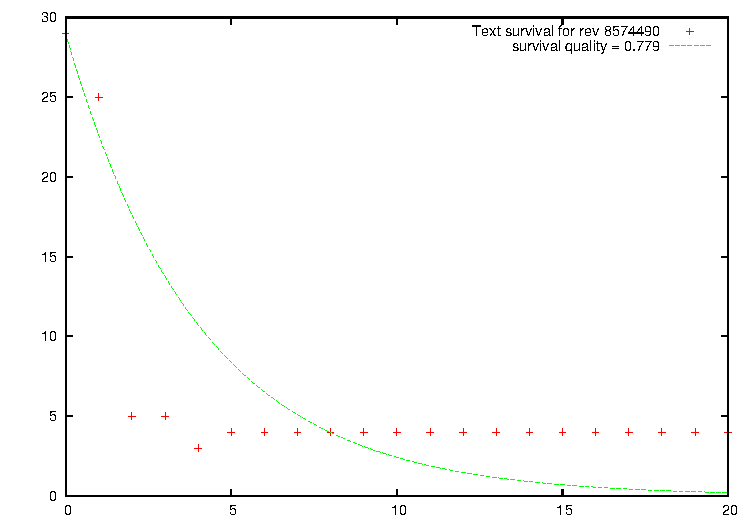
\includegraphics[width=0.8\textwidth]{part-F70-editquality/graph-TS-GeorgeWBush-8574490}}
\caption{The text survival graph for the text contributed early
        in the history of article \textit{George W.~Bush}.
	The graph also shows the text survival quality
	computed based on 20~revisions.
	}
\label{fig:ts-GeorgeWBush}
\end{figure}

\begin{figure}[tbph]
\centering
\framebox{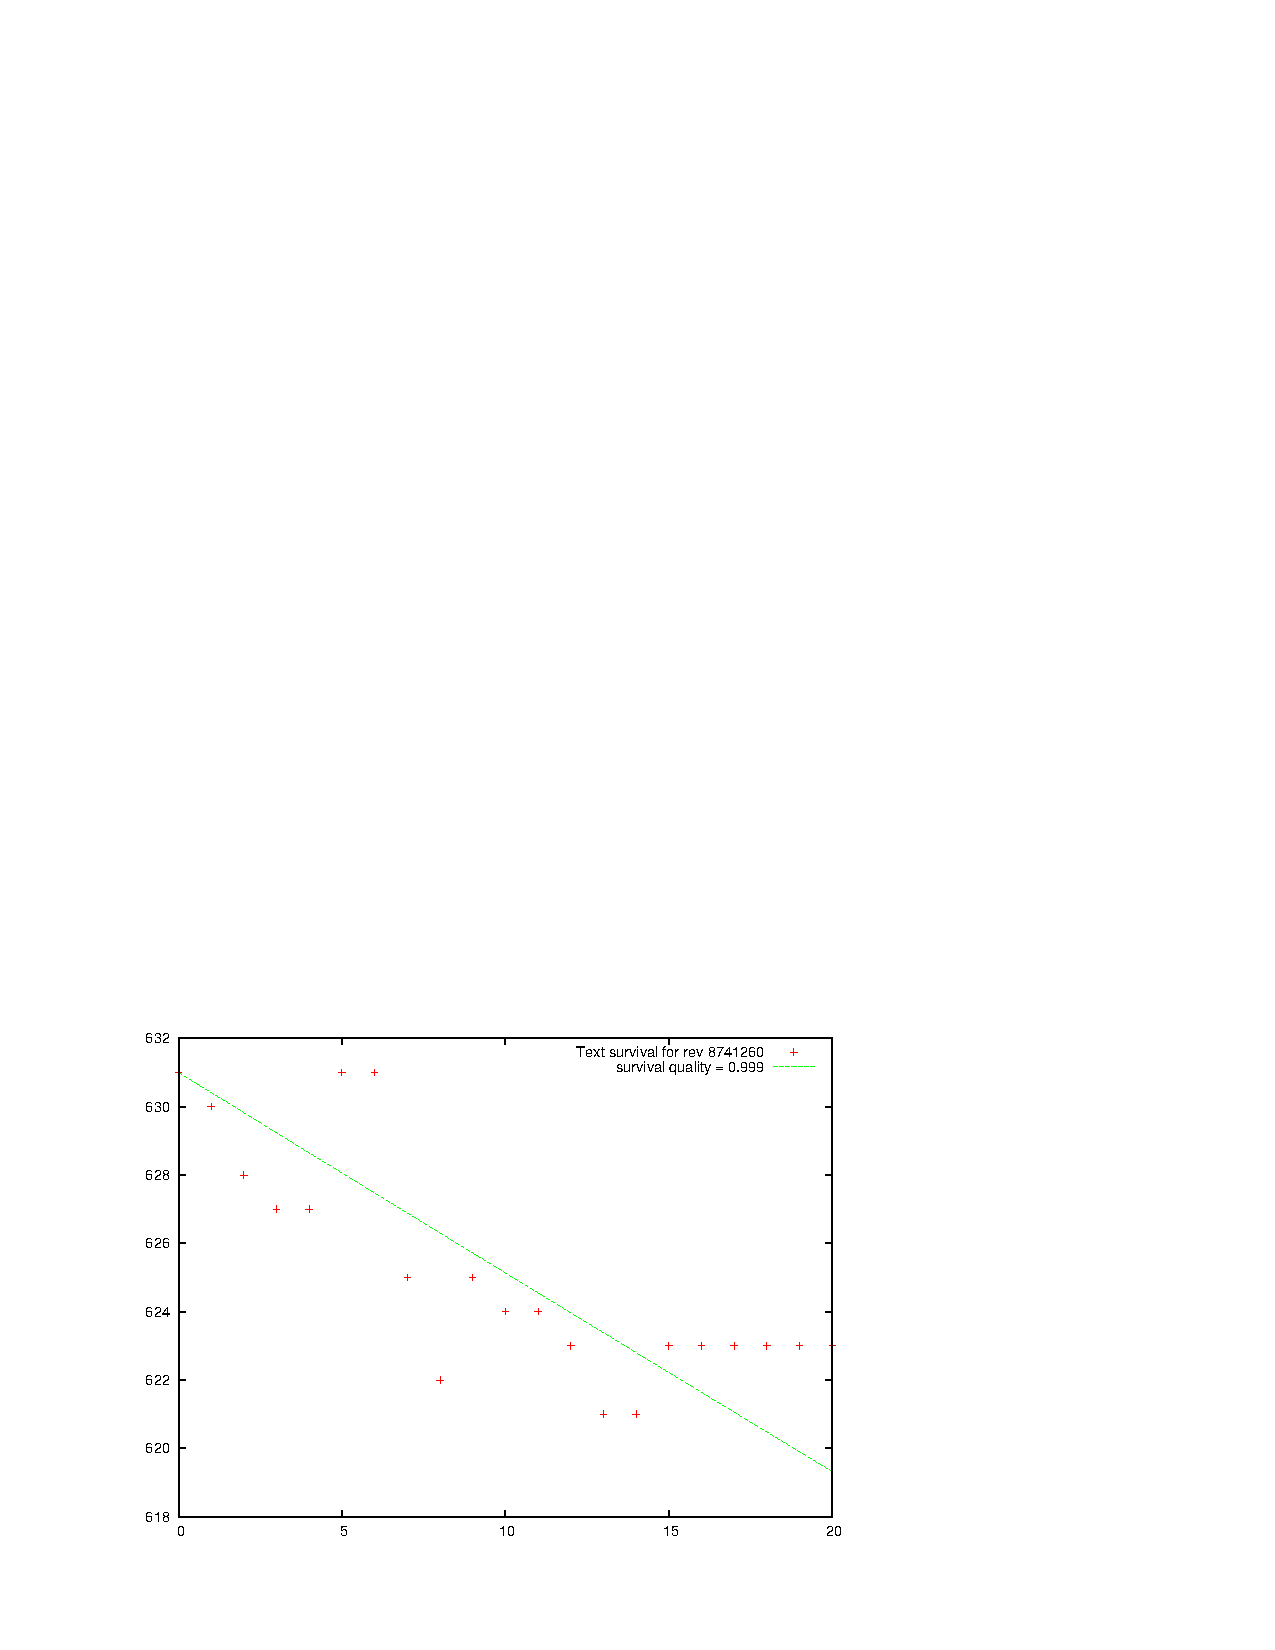
\includegraphics[width=0.8\textwidth]{part-F70-editquality/graph-TS-SantaCruzBeachBoardwalk}}
\caption{The text survival graph for the text initially contributed
	as part of the article \textit{Santa Cruz Beach Boardwalk}.
	The majority of the editing to the contributed text happens
	in the next few revisions, before the text stabilizes.
	The graph also shows the text survival quality
	computed based on 20~revisions.
	}
\label{fig:ts-SantaCruzBeachBoardwalk}
\end{figure}

The explanation for this discrepancy turns out to be a flaw in our
thinking about the original model.
While the text survival for contributions does seem to have an
exponential look to it, exponentials do not approach some fixed
non-zero value --- they approach zero.
In order to fit the curve we are describing, the last value
(in the case of the data shown in Figure~\ref{fig:ts-GeorgeWBush},
the amount of text that survives after the $20^{th}$ revision)
should be taken as the ``zero reference point'' which is subtracted
from all the values.
Applying our exponential curve fitting technique to these new values
will give a much better approximation to the data.
The problem with this better fit is that it changes the meaning of
a score of zero; instead of meaning that the text was immediately deleted,
a score of zero would mean that the text immediately reached its
final survival level.
In other words, we would be measuring how quickly the text stabilizes,
rather than how much agreement there was that the text belonged in
the article.

